\documentclass[12pt, a4paper]{article}
\usepackage{fullpage}
\usepackage{graphicx}
\usepackage{amsmath}
\usepackage{amssymb}
\usepackage[hidelinks]{hyperref}
\usepackage{listings}
\usepackage{epigraph}
\renewcommand{\epigraphsize}{\footnotesize}
\setlength{\epigraphwidth}{.5\textwidth}
\lstset{
  language = C,
  basicstyle = \ttfamily \small,
  numbers = left,
  numberstyle = \footnotesize,
  showstringspaces = false
}
\usepackage{times}

\title{601 Comprehensive II}
\author{Jeremy Kong}
\date{18 June 2017}

\begin{document}
\maketitle

\noindent A couple of quick notes:
\begin{itemize}
\item I'd intend for the timelimit for this paper to be 3 hours and 20 minutes (200 minutes total).
\item This question was constructed by a student at Imperial College London, and is not intended to be representative of actual examination questions for any specific course at Imperial.
\item The material students have learned from the compulsory modules in first and second year should be sufficient to answer all questions.
\item Each question is worth 20 marks; the maximum mark is thus 100.
\item The questions are roughly arranged in what I think is difficulty order. Also, \textit{within each question} the difficulty generally increases as you progress from one part to the next.
\item This exam is \textbf{hard} and intended to be hard. The author obtained an average of $92.9$ percent in his second year at Imperial, but would only expect to score about $70$ on this exam.
\end{itemize}

\newpage
$\:$
\newpage 

\section{To A Brighter Day}
\epigraph{Cause if we lost our minds, and we took it way too far \\
I know we'd be alright, I know we would be alright \\
If you were by my side, and we stumbled in the dark \\
I know we'd be alright, I know we would be alright --
}{\textit{``There's Nothing Holding Me Back", Shawn Mendes}}

\noindent \textsc{Light Up} (also called \textsc{Akari}) is a logic puzzle first published 
by Nikoli \cite{lightup}. The puzzle is played on a two-dimensional plane and involves an 
$n \times n$ matrix of cells. An example of a \textit{very} simple puzzle and its solution
are shown below:
\begin{center}
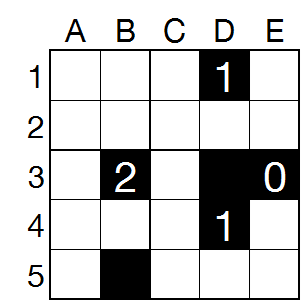
\includegraphics[scale=0.7]{lightsout1.png}
\hspace{3cm}
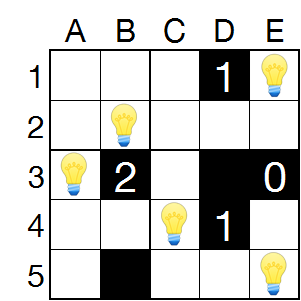
\includegraphics[scale=0.7]{lightsout2.png}
\end{center}

Players seek to place lightbulbs on some squares, subject to the following constraints:
\begin{itemize}
\item A lightbulb emits light in the four cardinal directions (north, south, east
and west). Light travels in a straight line until it hits a block (black square), or
the edge of the grid.
\item Lightbulbs can only be placed in white squares. They must light up all white squares
in the grid. The square a lightbulb itself is on is considered to be lit.
\item Lightbulbs must \textit{not} shine on each other. (However, a single square 
can be illuminated by multiple lightbulbs, as long as the bulbs
themselves don't light each other.)
\item Some black squares are marked with \textit{clues}. A clue indicates the number of
lightbulbs adjacent to the relevant black square (but \textit{only} in the four cardinal
directions).
\end{itemize}

For example, the simple puzzle above may be solved using the following reasoning.
\begin{itemize}
\item Neither E2 or E4 can contain a lightbulb (because of the 0 in E3).
\item The entire grid must be lit -- so E5 must contain a lightbulb, as must E1.
\item C1 and D2 cannot contain lightbulbs (because of the 1 in D1). Also, C5 and D5
cannot contain lightbulbs (because the bulb on E5 shines there).
\item So C4 must have a lightbulb to satisfy the 1 in D4.
\item This means C3 and B4 cannot contain lightbulbs; but to satisfy the 2 in B3,
A3 and B2 must contain lightbulbs. We've now lit every square, so we are done.
\end{itemize}

S

\newpage
\begin{thebibliography}{9}
\bibitem{lightup}
``Rules of Akari puzzle." Accessed 18 June 2017. $<$\url{http://www.nikoli.com/en/puzzles/bijutsukan/rule.html}$>$

\bibitem{orleans}
Bernstein, Philip A., et al. ``Orleans: Distributed Virtual Actors for Programmability and Scalability."
\end{thebibliography}

\newpage

\end{document}